%!TEX root = ../final_report.tex

\textit{Clearly describe your experimental protocols. If you are using training and test data, report the numbers of training and test images. Be sure to include example output figures. Quantitative evaluation is always a big plus (if applicable). If you are working with videos, put example output on YouTube or some other external repository and include links in your report.}


\subsection{Framework}
This project is implemented based on Keras framework \cite{Chollet2015_keras}, which is a modular neural network library. The library is written in Python and can run on top of Theano or TensorFlow. In this project, we propose to use Theano backend \cite{theano2016} for implementation.

Since we need to use pretrained weights from AlexNet, our system has to be able to load this network. However, AlexNet is provided under caffemodel format, which is used in CaffeNet-based deep learning networks \cite{Jia2014_caffe}. The problem is original Keras framework does not allow to load caffemodel directly. Therefore, we use a modified version of Keras, provided by Sol\`{a} \cite{Sola2016}. This version includes a fully functional Keras framework with an additional package for converting from caffemodel to keras format.



\subsection{Implementation}
The project contains 4 main modules: data processor, model architecture, model training, and model testing.

\subsubsection{Data Processor}
The module takes care of loading and preprocessing input data. The input data are cropped with respect to the ground truth segmentation mask beforehand, as showed in Figure \ref{fig:img_cropped}. For preprocessing task, inputs undergo the procedure introduced in Section \ref{subsec:preprocessing}: images are resized efficiently to the size of 227x227 (based on Equation \ref{equ:rescale}) and depth maps have an additional step of colorizing. 

For data loading, the module receive a batch of image, a dictionary list (containing all possible categories), and location of data. Since the amount of data is significant, we cannot load everything at the same time, therefore batch processing is necessary. Based one the naming format of each sample in the batch (Section \ref{subsec:dataset}), we can easily figure out which category that sample belong to and construct the label vector according to the given dictionary
as seen in Equation \ref{equ:label}. Since we are using pretrained weights from AlexNet to train the network, it is essential to remove the mean image of ImageNet from every input after loading.

\subsubsection{Model Architecture}
This module creates the architecture for the stream and fusion networks. Common Keras-based systems are implemented based on Sequential model, which allows adding layers in a sequential manner. Such scheme of architecture is actually found in popular network, such as AlexNet \cite{Krizhevsky2012_alexnet}, VGG \cite{Simonyan2014_vgg}. However, such architecture faces the problem of constructing fusion layer. Although Keras provides layer called Merge layer to concatenate different sources of input, it does not work well with Sequential model, making it impossible to load networks after training. To overcome this problem, we use Graph models instead, which offers more flexibility but still retains core functionalities as in Sequential models.

The module has two main parts: the first one replicates the network architecture of AlexNet and the second one constructs the fusion network from stream models. 

\subsubsection{Model Training}

\subsubsection{Model Testing}

\subsection{Experimental Results}

Experiment Setup (train - eval - test)

\begin{figure}[htbp]
	\centering
	\begin{subfigure}[b]{0.45\linewidth}
		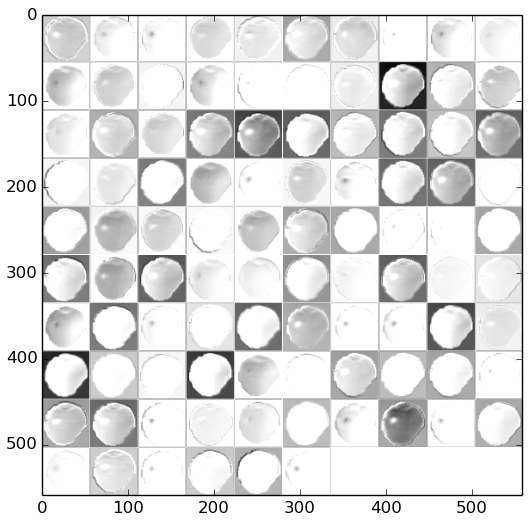
\includegraphics[width=\textwidth]{img/relu1_rgb.png}
		\caption{Activation of ReLU1 layer for RGB image}
	\end{subfigure}   	
	\begin{subfigure}[b]{0.45\linewidth}
		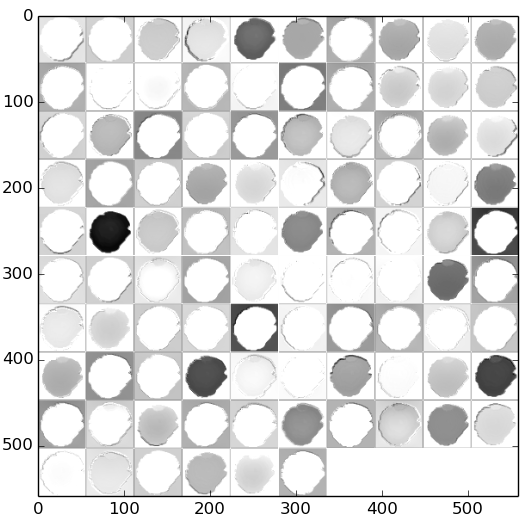
\includegraphics[width=\textwidth]{img/relu1_dep.png}
		\caption{Activation of ReLU1 layer for Depth image}
	\end{subfigure}
	
	\begin{subfigure}[b]{0.45\linewidth}
		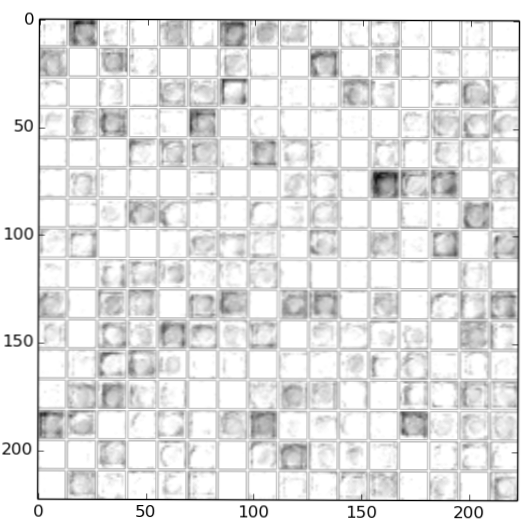
\includegraphics[width=\textwidth]{img/relu5_rgb.png}
		\caption{Activation of ReLU5 layer for RGB image}
	\end{subfigure}   	
	\begin{subfigure}[b]{0.45\linewidth}
		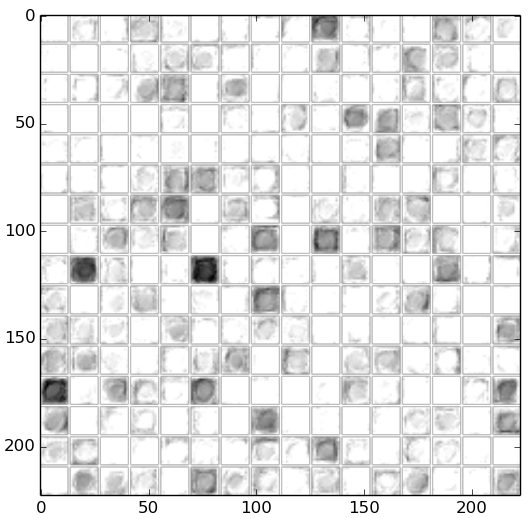
\includegraphics[width=\textwidth]{img/relu5_dep.png}
		\caption{Activation of ReLU5 layer for Depth image}
	\end{subfigure}
	\caption{Visualization of intermediate results on the first and fifth ReLU layers on both RGB and depth images of an apple.}
	\label{fig:intermediate_result}
\end{figure}

\begin{table}[htbp]
	\centering
	\caption{Recognition accuracy on reduced (5 categories) and full dataset (51 categories) for RGB stream, depth stream, and fusion network}
	\label{tab:result}
	\begin{tabular}{|c|c|c|c|}
		\hline
		& RGB stream & Depth stream & RGB-D fusion network \\ \hline
		Reduced dataset & 68.26\% & 74.43\% & 56.52\% \\ 
		Full dataset & 68.93\% & 79.19\% & 8.07\% \\ 
		Full dataset with refactored fusion layers & 68.93\% & 79.19\% & 17.34\% \\ \hline
	\end{tabular}
\end{table}

\begin{figure}[htbp]
	\centering
	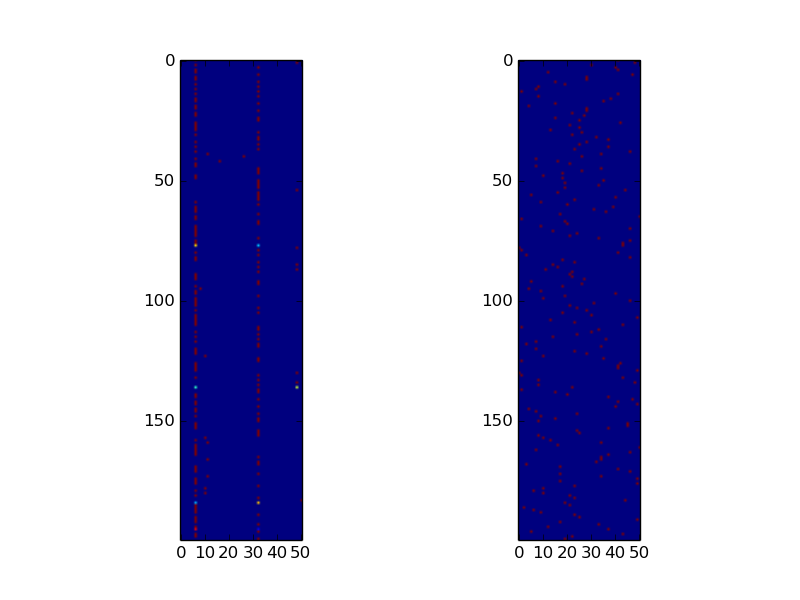
\includegraphics[width=\textwidth]{img/prediction.png}
	\caption{Prediction results with unfactored fusion layer.}
	\label{fig:prediction}
\end{figure}

\begin{figure}[htbp]
	\centering
	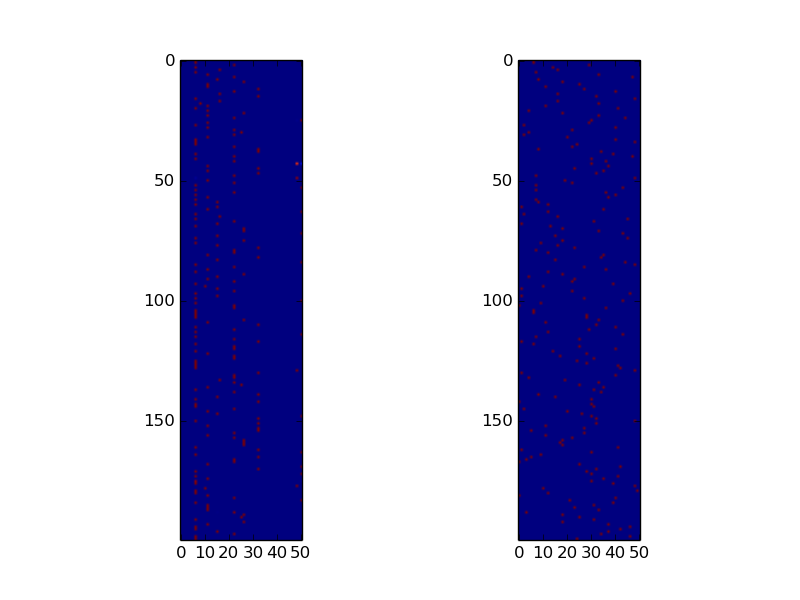
\includegraphics[width=\textwidth]{img/prediction_refactored.png}
	\caption{Prediction results with refactored fusion layer.}
	\label{fig:prediction_refactored}
\end{figure}